\def\s{\section*}
\def\ss{\subsection*}
\def\sp{\hspace{3 mm}}
\def\ind{\!\perp\!\!\!\perp}
\def\m{\mid}
\def\nl{ \\ = \sp &}
\newcommand{\eq}[1]{\begin{align*}&{#1}\end{align*}}
\renewcommand{\ss}[1]{\subsection*{#1}}
\renewcommand{\P}[1]{\s{Problem #1}}
\def\ra{\rightarrow}
\def\la{\leftarrow}
\def \pb{\newline\newline}
\newcommand{\pic}[2]{\begin{figure}[H]
  \includegraphics[width=\linewidth]{#2}
  \caption{#1}
  \label{fig:net}
\end{figure}}

\documentclass[10pt,a4paper]{article}
\usepackage[utf8]{inputenc}
\usepackage{amsmath}
\usepackage{parskip}
\usepackage{amsfonts}
\usepackage{lmodern}
\usepackage{physics}
\usepackage{float}
\usepackage{graphicx}
\usepackage{amssymb}
\author{Hugh Zhang}
\title{CS 228 Problem Set 1}
\date{\today}
\begin{document}
\maketitle

\P 1

We want to compute $P(C \mid v_1\dots v_k)$. For our purposes, our sampler Q is uniform on the possible, so assuming a permutation x' is possible to reach from a state x, then the probabilities are equal. Thus, we can cancel the Qs out.

Acceptance probability is

\begin{align*}
& A(c' \mid c, v_1 \dots v_k) \nl min (1, \frac{P(c' \mid v_1 \dots v_k )Q(c \mid x', v_1 \dots v_k)}{P(c \mid v_1 \dots v_k )Q(c' \mid x, v_1 \dots v_k}) \nl
min (1, \frac{P(c' \mid v_1 \dots v_k )}{P(c \mid v_1 \dots v_k )})
\end{align*}

How do we calculate \[
\frac{P(c' \mid v_1 \dots v_k)}{P(c \mid v_1 \dots v_k)}
\]

\begin{align*}
& \frac{P(c' \mid v_1 \dots v_k)}{P(c \mid v_1 \dots v_k)} \nl
\frac{P(c', v_1 \dots v_k)}{P(c, v_1 \dots v_k)} \nl
\frac{P(v_1 \dots v_k \mid c') P(c')}{P(v_1 \dots v_k \mid c) P(c)}
\end{align*}

We are given $P(v_1 \dots v_k \mid C) = \prod_{v_1 \dots v_k} P(v_i \mid C)$, and although we don't quite know P(c), we are given the assumption that it is uniform a priori, so for our approximation it cancel out.

\ss {1.2}

The samples are directly from $P(C \mid v_1 \dots v_k)$. Thus,
\[P(C_i = k \mid v_1 \dots v_k) = \frac{\sum_{m=1}^M 1(C_i[m]==k)}{M}
\], or in English, just count the number of times you see it in the sample and divide it by the total number of samples.

\ss {1.3}

Gibbs sampling does not work. When we sample C, we take two elements $C_i$ and $C_j$ and swap them. If we were to try to Gibbs sample this and try to sample each $C_i$ independently and in order for all i, we would get invalid samples that were not permutations.

\P 2

From lecture, we have.

\begin{align*}
& \log P(y_i \mid x_i, \theta) \nl \log(\frac{1}{Z(x^i, \theta)} \prod_{n \in N} exp(\theta_n f_n(x^i,y_n^i)))) \nl
\sum_{n \in N} \theta_n f_n(x^i,y_n^i)) - log(Z(x^i, \theta)) \nl
\sum_{n \in N} \theta_n f_n(x^i,y_n^i)) - log \sum_y exp(\theta_n * f_n(y,x^i))
\end{align*}

Since the likelihood is just the log of the probability summed over all the data, letting M be the number of examples in D, we have

\begin{align*}
& g(\theta, D) = (1-\alpha)\ell_{Y \mid X}(\theta, D) + \alpha\ell_{X \mid Y}(\theta,D)
\end{align*}

Where as per above,

\begin{align*}
&\ell_{Y \mid X}(\theta, D) = \sum_i^M (\sum_{n \in N} \theta_n f_n(x_n^i,y_n^i)) - \log \sum_y exp(\theta_n * f_n(y_n,x_n^i))) \\ \sp &
\ell_{X \mid Y}(\theta, D) = \sum_i^M (\sum_{n \in N} \theta_n f_n(x_n^i,y_n^i)) - \log \sum_x exp(\theta_n * f_n(y_n^i,x_n)))
\end{align*}

I don't quite want to substitute everything in, but the equation is right there :).

\ss{2.2}

We want to calculate 

\def\t{\pdv{\theta}}

\begin{align*}
& \pdv{\theta} g(\theta,D) \nl
(1-\alpha)\t\ell_{Y \mid X}(\theta, D) + \alpha\t\ell_{X \mid Y}(\theta,D)
\end{align*}

We calculate 
\begin{align*}
& \t\ell_{Y \mid X}(\theta, D) \nl 
\t \sum_i^M (\sum_{n \in N} \theta_n f_n(x_n^i,y_n^i) - log \sum_n \sum_y exp(\theta_n * f_n(y_n,x_n^i))) \nl 
\sum_i^M (\sum_{n \in N} f_n(x_n^i,y_n^i) - \t\log \sum_y exp(\theta_n * f_n(y_n,x_n^i))) \nl 
\sum_i^M (\sum_{n \in N} f_n(x_n^i,y_n^i) - \frac{1}{ \sum_y exp(\theta_n * f_n(y_n,x_n^i)))} * \t ( \sum_y exp(\theta_n * f_n(y_n,x_n^i)))) \nl 
\sum_i^M (\sum_{n \in N} f_n(x_n^i,y_n^i) - \frac{ \sum_y exp(\theta_n * f_n(y_n,x_n^i)) * f_n(y_n,x_n^i))}{ \sum_y exp(\theta_n * f_n(y_n,x_n^i)))} \nl 
\sum_i^M (\sum_{n \in N} f_n(x_n^i,y_n^i) - \frac{ \sum_y exp(\theta_n * f_n(y_n,x_n^i))) * f_n(y_n,x_n^i))}{Z(\theta, x^i)} \nl
\sum_i^M (f(x^i,y^i) - \sum_y P(y,x^i) f(y,x^i)) \nl
M*E_Q[f(x,y)] - M*E_Q [E_{p(y \mid x)}[f(x^i,y^i)]]
\end{align*}

 Where Q is the distribution that you got while sampling 
 
\begin{align*}
 & M(E_Q[f(x,y)] - E_Q[E_{p(y \mid x)}[f(x,y)]] - \alpha E_Q[f(x,y)] + \alpha E_Q[E_{p(y \mid x)}[f(x,y)]] \\  + & \alpha E_Q[f(x,y)] - E_Q[E_{p(x \mid y)}[f(x,y)]]) \nl M(E_Q[f(x,y)] - E_Q[E_{p(y \mid x)}[f(x,y)]] + \alpha E_Q[E_{p(y \mid x)}[f(x,y)]] - \alpha E_Q[E_{p(x \mid y)}[f(x,y)]])
\end{align*}

\P 3

E step:

Let $A = \abs{Val(C)}$ and $B_i = \abs{Val(X_i)}$

For each C, we compute

\begin{align*}
& Q(C \mid X) = \frac{P(X \mid C) * P(C)}{\sum_C P(X \mid C) * P(C)} \nl
\frac{\theta_{x\mid c}^0 * \theta_C^0}{\sum_C \theta_{x\mid c}^0 * \theta_C^0} \nl
\frac{\frac{1}{B}\frac{1}{A}}{A*\frac{1}{B}\frac{1}{A}} \nl
\frac{1}{A}
\end{align*}

So $Q^1(C \mid X)$ is just uniform over C, as we expect.

M step:

We want to set. 

\begin{align*}
& \theta^1 = \arg\max_{\theta} \sum_D \sum_C Q^1(C \mid X) \log P(C, X, \theta) \nl
\arg\max_{\theta} \sum_D \sum_C \frac{1}{A} \log \theta_C \theta_{x\mid c} \nl
\arg\max_{\theta}( \sum_D \sum_C \log \theta_C + \sum_D \sum_C \log\theta_{x\mid c} )
\end{align*}

$\frac{1}{A}$ has no bearing on maximizing the parameters. Another way of putting the above is that C has to be uniform at the end, because we have no information for which way to bias C. Thus, $\theta_C$ remains constant. According to the lecture notes, the proper way to maximize $\log\theta_{x\mid c}$ is to set it to the weighted observed counts in the data.

\begin{align*}
& \theta_C = \frac{1}{A} \\
& \theta_{x\mid c} = \frac{\sum_D P(c,x)}{\sum_D \sum_x P(c,x)} = \frac{cnt(x)}{M}
\end{align*}

Since C gives us no information, we it is essentially unifrom MLE and where cnt(x) is how many times x appears in the training data.

To show that it converges there and no longer changes, we hallucinate C again, and it will be uniform since we have no other information on it.

\begin{align*}
& Q(C \mid X) = \frac{P(X \mid C) * P(C)}{\sum_C P(X \mid C) * P(C)} \nl
\frac{\theta_{x\mid c}^0 * \theta_C^0}{\sum_C \theta_{x\mid c}^0 * \theta_C^0} \nl
\frac{\frac{1}{B}\frac{1}{A}}{A*\frac{1}{B}\frac{1}{A}} \nl
\frac{1}{A}
\end{align*}

And since $P(C \mid X)$ is as in step 1, nothing will update for the parameters, so this is the final distribution.

\P 4

Let A denote the set of variables not in either Y or Y's markov blanket. I'm going to split up $Y_M(i,j)$ to include the 2-4 neighboring Y variables, and separately include $x_{ij}$, which would ordinarily be in Y's markov blanket. The general gist is that everything in A cancels out.

\begin{align*}
& P(y_{ij} \mid y_{M(i,j)}) = \frac{P(y_{ij}, y_{M(i,j)})}{ P(y_{M(i,j)}))} \nl
\frac{\sum_A P(y_{ij}, y_{M(i,j)}, A)}{ \sum_A \sum_{y_{ij}} P(y_{ij} y_{M(i,j)}),A)} \nl
\frac{\sum_A exp(\eta \sum_N \sum_M y_{ij}x_{ij} +  \beta \sum_{edges} y_{ij}y_{i'j'})}{ \sum_A \sum_{y_{ij}} exp(\eta \sum_N \sum_M y_{ij}x_{ij} +  \beta \sum_{edges} y_{ij}y_{i'j'}) } \nl 
\frac{exp(\eta y_{ij}x_{ij} + \beta \sum_{Y_{M(i,j)}} y_{ij}y_{i'j'}) * \sum_A exp(\eta \sum_A y_a x_a + \beta \sum_{restofedges} y_{ij}y_{i'j'})}{\sum_{y_{ij}} exp(\eta y_{ij}x_{ij} + \beta \sum_{Y_{M(i,j)}} y_{ij}y_{i'j'}) * \sum_A exp(\eta \sum_A y_a x_a + \beta \sum_{restofedges} y_{ij}y_{i'j'})} \nl
\frac{exp(\eta y_{ij}x_{ij} + \beta \sum_{Y_{M(i,j)}} y_{ij}y_{i'j'})}{\sum_{y_{ij}} exp(\eta y_{ij}x_{ij} + \beta \sum_{Y_{M(i,j)}} y_{ij}y_{i'j'})}
\nl \frac{exp(\eta y_{ij}x_{ij} + \beta \sum_{Y_{M(i,j)}} y_{ij}y_{i'j'})}{exp(\eta x_{ij} + \beta \sum_{y_{i'j'} \in Y_{M(i,j)}} y_{i'j'}) + exp(-\eta x_{ij} - \beta \sum_{y_{i'j'} \in Y_{M(i,j)}} y_{i'j'})}
\end{align*}

Thus, 

\begin{align*}
& P(y_{ij} = 1 \mid Y_{M(i,j)}, x_{ij}) \nl \frac{exp(\eta x_{ij} + \beta \sum_{Y_{M(i,j)}} y_{i'j'})}{exp(\eta x_{ij} + \beta \sum_{y_{i'j'} \in Y_{M(i,j)}} y_{i'j'}) + exp(-\eta x_{ij} - \beta \sum_{y_{i'j'} \in Y_{M(i,j)}} y_{i'j'})} \nl
\frac{1}{1+ exp(-2\eta x_{ij} - 2\beta \sum_{y_{i'j'} \in Y_{M(i,j)}} y_{i'j'})}
\end{align*}

Which is a sigmoid function.

\ss {4.2}

You are given the X's and randomly initialize the Ys. Then, go through the Y's in order and draw from the $P(y_{ij} = 1 \mid Y_{M(i,j)}, x_{ij})$ that we gave above (using the newest values of Y that we just got if necessary). When you have gone through all the Y's you have gone through one "iteration" of Gibbs Sampling. After burning through the burn in samples, Gibbs Sampling guarantees that we converge to $P(Y \mid X)$ eventually because this is clearly ergodic.

Irreducible: You can get to any Y with sufficient luck because any sample is possible.

Aperiodic: You can hit any Y in one "iteration" of Gibbs if you sample the right pixel at each step, since each pixel has a non zero chance of hitting 0/1 each sample.

\ss {4.3}

All three converge to the same approximate energy: -214000. The chains eventually end up mixing for all three starts, which indicates that our Gibbs sampling is not really getting stuck and is doing the right job. The burn in period for the same and the random seems sufficient, since the burn in samples seem mixed in themselves before we start the real samples. With the logneg graph, it is less clear, since the graph hasn't clearly started mixing yet and the beginning of our sample might be not quite $P(Y \mid X)$. A touch longer burn in might be safer.

\pic{Log Neg}{pa4/log_neg.png}
\pic{Log Same}{pa4/log_same.png}
\pic{Log Rand}{pa4/log_rand.png}



\ss{4.4}

Correct pixels for 10: 84454
Correct pixels for 20: 84072
Total: 84960

Accuracy 10: 99.4 or .6 error
Accuracy 20: 98.95 or 1.05 error

\begin{figure}[!htb]
\minipage{0.32\textwidth}
  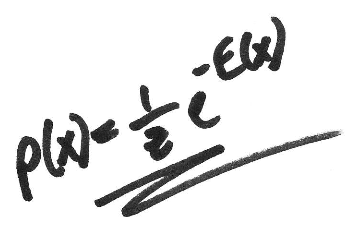
\includegraphics[width=\linewidth]{pa4/orig.png}
  \caption{Original}\label{fig:awesome_image1}
\endminipage\hfill
\minipage{0.32\textwidth}
  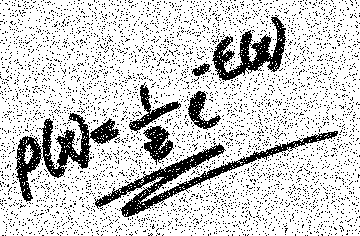
\includegraphics[width=\linewidth]{pa4/noisy_10.png}
  \caption{Noisy 10}\label{fig:awesome_image2}
\endminipage\hfill
\minipage{0.32\textwidth}%
  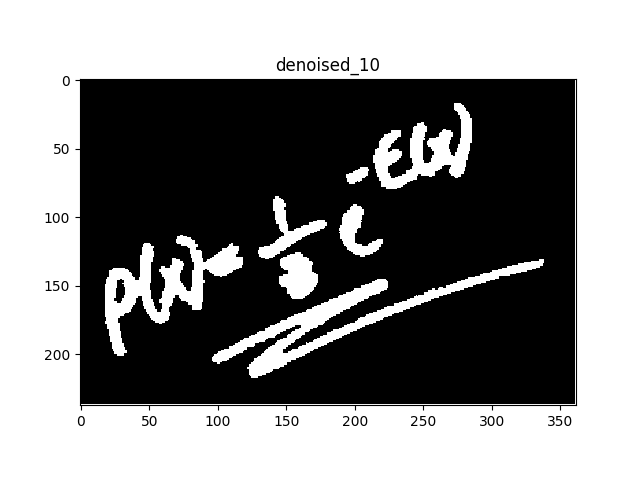
\includegraphics[width=\linewidth]{pa4/denoised_10.png}
  \caption{Denoised}\label{fig:awesome_image3}
\endminipage
\end{figure}

\begin{figure}[!htb]
\minipage{0.32\textwidth}
  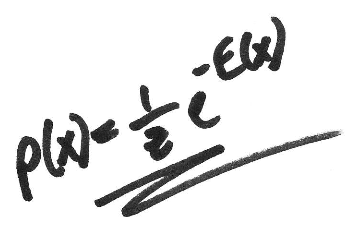
\includegraphics[width=\linewidth]{pa4/orig.png}
  \caption{Original}\label{fig:awesome_image1}
\endminipage\hfill
\minipage{0.32\textwidth}
  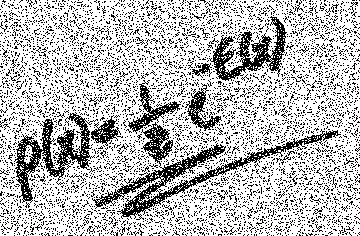
\includegraphics[width=\linewidth]{pa4/noisy_20.png}
  \caption{Noisy 20}\label{fig:awesome_image2}
\endminipage\hfill
\minipage{0.32\textwidth}%
  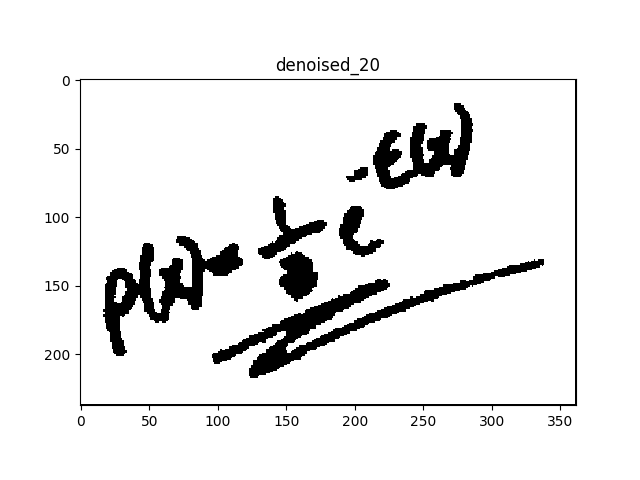
\includegraphics[width=\linewidth]{pa4/denoised_20.png}
  \caption{Denoised}\label{fig:awesome_image3}
\endminipage
\end{figure}

\ss{4.5}

Correct pixels for 10: 84340
Correct pixels for 20: 82995
Total: 84960

Accuracy 10: 99.27 or 0.73 error
Accuracy 20: 97.69 or 2.31 error

Caveats: The accuracies vary slightly based on what you do for ties and what order you iterate through the photo. But in general, it performs similarly but slightly worse to Gibbs sampling. This is because, our version of Gibbs sampling is doing a very similar algorithm with $\eta$ and $\beta$ both being 1, you are essentailly looking at your neighbors and seeing which direction they want you to go. The difference is that Gibbs sampling is probabilistic so it explores more and doesn't get suck on a suboptimal photo (although notice that it does require more iterations 1100 to 30)

\pic{Bad Algo Restored 10}{pa4/denoised_dumb_10.png}
\pic{Bad Algo Restored 20}{pa4/denoised_dumb_20.png}

\ss{4.6}

Both normalish distributions. Noisy 10 has slightly less pixels on average (703 ish?) compared to Noisy 20 (718 ish?), which is better, because the original image has 680 pixels in that rectangle which is lower than either of them

\pic{Noisy 10 picture hisogram}{pa4/noisy10histo.png}
\pic{Noisy 20 picture hisogram}{pa4/noisy20histo.png}

\end{document}